\subsubsection{Exercise}

Our objective now is to determine two inputs ($u_1, u_2$) in order to reach $60\%$ of full tank in tank $1$ and $2$.

Once the values for each parameters $a_{1 \leq i \leq 4}$ and $k_{1,2}$ are known, the equilibrium system from exercice 2.1.2 can be solved in order to find the values of $h_3^0,h_4^0,u_1,u_2$ (inputs are $h_1^0,h_2^0$).  

The system is the following:
$$
    \footnotesize
\left[
    \begin{array}{cccc}
        \gamma_1 k_1 & 0 & a_3 \sqrt{2g} & 0 \\
        0 & \gamma_2 k_2 & 0 & a_4 \sqrt{2g} \\
        0 & (1-\gamma_2) k_2 & -a_3 \sqrt{2g} & 0 \\
        (1-\gamma_2) k_1 & 0 & 0 & -a_4 \sqrt{2g} \\
    \end{array}
\right]
\left[
    \begin{array}{c}
        u1 \\ u2 \\ \sqrt{h_3^0} \\ \sqrt{h_4^0}
    \end{array}
\right]
=
\left[
    \begin{array}{c}
        a_1 \sqrt{2gh_1^0} \\
        a_2 \sqrt{2gh_2^0} \\
        0 \\
        0 \\
    \end{array}
\right]
$$

Therefore solving this linear with $h_1^0$ and $h_2^0$ as parameters compute the values of $u_1$ and $u_2$. 
Using this method with the two sets of parameters (Minimum and non-minimum case) leads to the results displayed in Figure \ref{manualcontrol}.

The transient time is reported in the following table:

\begin{center}
    \footnotesize
\begin{tabular}{|cc|}
    \hline
    \multicolumn{2}{|c|}{Transient time} \\
    \hline
    Mininum case & $98$s \\
    Non-mininum case & $55$s \\
    \hline
\end{tabular}
\end{center}

\begin{figure}[h!t]
        \centering
        \begin{subfigure}[b]{0.45\columnwidth}
                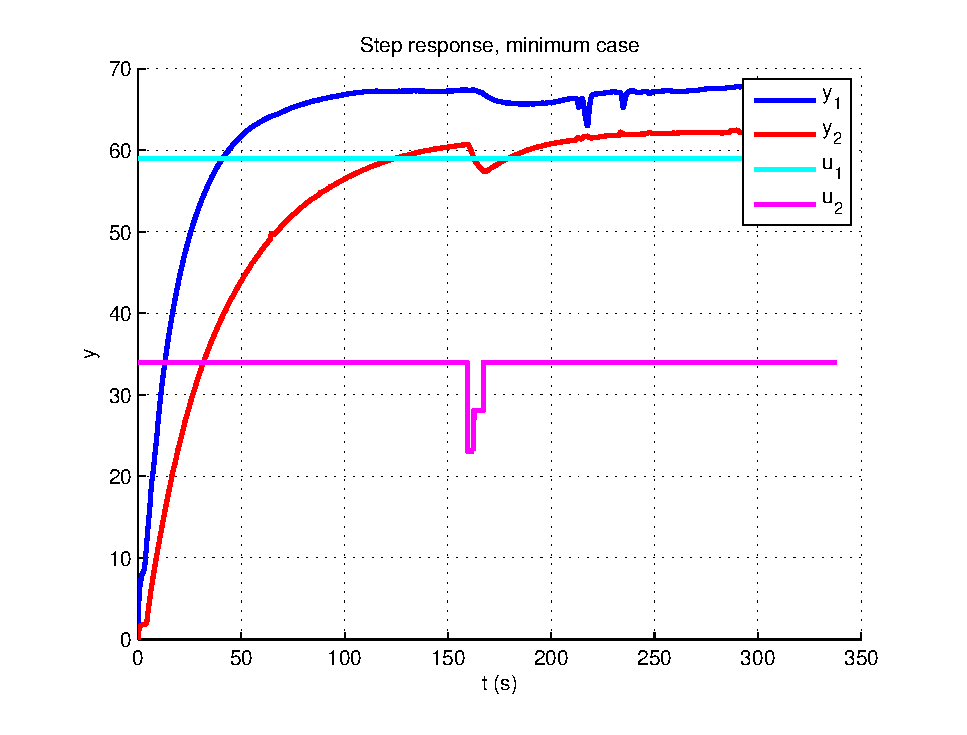
\includegraphics[width=\columnwidth]{fig/manualcontrolmin.eps}
                \caption{$u_1 = 59\%, u_2 = 34\%$ \\ $h_1^0 = h_2^0 = 15cm$}
        \end{subfigure}
        \begin{subfigure}[b]{0.45\columnwidth}
                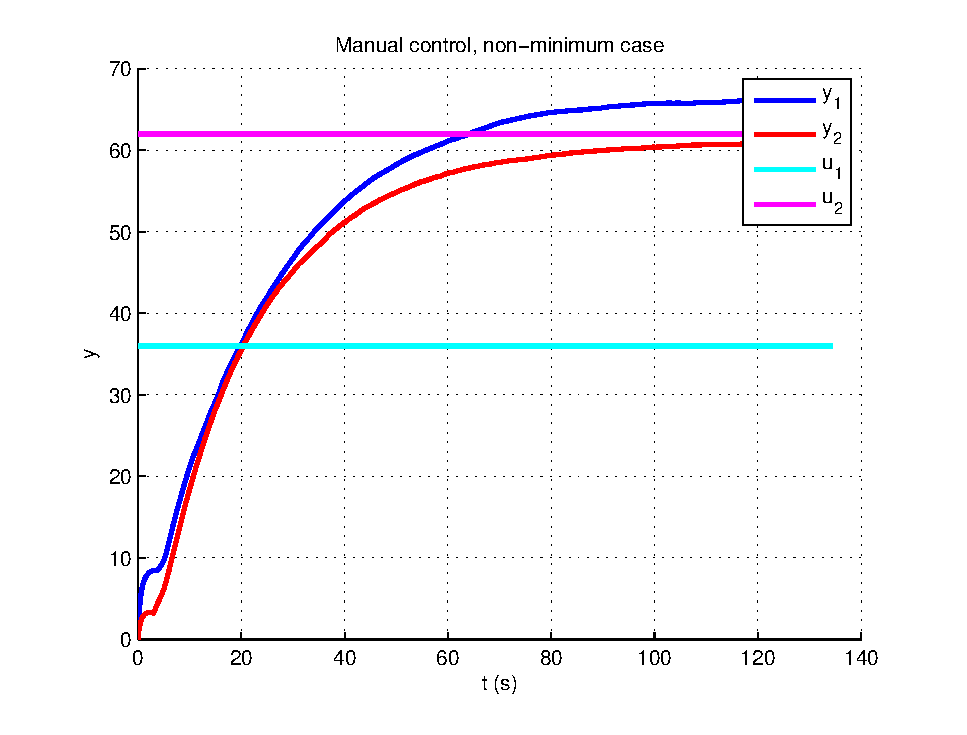
\includegraphics[width=\columnwidth]{fig/manualcontrolnonmin.eps}
                \caption{$u_1 = 36\%, u_2 = 62\%$ \\ $h_1^0 = h_2^0 = 15cm$}
        \end{subfigure}
        \caption{Manual control of $h_1^0, h_2^0$}
        \label{manualcontrol}
\end{figure}



The two curves do not merge after the transient time. Indeed, the two sensors present different offset (\emph{i.e} $h_1 = 0$ do not lead to exactly $y_1 = 0$).
However, this offset is constant for each sensor and after verification the same level of water have been reached in both tanks.

